% Created 2019-09-20 Пт 15:13
% Intended LaTeX compiler: pdflatex
\documentclass[11pt]{article}
\usepackage[utf8]{inputenc}
\usepackage[T1]{fontenc}
\usepackage{graphicx}
\usepackage{grffile}
\usepackage{longtable}
\usepackage{wrapfig}
\usepackage{rotating}
\usepackage[normalem]{ulem}
\usepackage{amsmath}
\usepackage{textcomp}
\usepackage[export]{adjustbox}
\usepackage{amssymb}
\usepackage{capt-of}
\usepackage{hyperref}
\usepackage[T2A]{fontenc}
\usepackage[a4paper,left=3cm,top=2cm,right=1.5cm,bottom=2cm,marginparsep=7pt,marginparwidth=.6in]{geometry}
\usepackage{cmap}
\usepackage[russian]{babel}
\usepackage{xcolor}
\usepackage{listings}
\author{АВТОР}
\lstset{
  language = Prolog,
  literate = {-}{-}1, % <------ trick!
}
\date{\today}
\title{}
\hypersetup{
 pdfauthor={АВТОР},
 pdftitle={},
 pdfkeywords={},
 pdfsubject={},
 pdfcreator={Emacs 26.1 (Org mode 9.1.9)}, 
 pdflang={Russian}}
\begin{document}

\large
\thispagestyle{empty}
\begin{center}
\textbf{Санкт-Петербургский Национальный Исследовательский}\\
\textbf{Университет Информационных Технологий, Механики и Оптики}\\
\textbf{Факультет Программной Инженерии и Компьютерной Техники}\\
\end{center}
\vspace{1em}
\begin{center}

\includegraphics[width=120px]{../../../itmo-logo.png}
\end{center}
\LARGE
\vspace{5em}
\begin{center}
\textbf{Вариант № 9005}\\
\textbf{Лабораторная работа № 1}\\
\Large
\textbf{по дисциплине}\\
\LARGE
\textbf{\emph{'Основы профессиональной деятельности'}}\\
\end{center}
\vspace{11em}
\large
\begin{flushright}
\textbf{Выполнил:}\\
\textbf{Студент группы P3113}\\
\textbf{\emph{Куперштейн Дмитрий;} : 269359}\\
\textbf{Преподаватель:}\\
\textbf{\emph{ПЕРМИНОВ ИЛЬЯ ВАЛЕНТИНОВИЧ}}\\
\end{flushright}
\vspace{4em}
\large
\begin{center}
\textbf{Санкт-Петербург 2019 г.}
\end{center}
\pagebreak{}

\lstset{basicstyle=\ttfamily,
  showstringspaces=false,
  commentstyle=\color{red},
  keywordstyle=\color{blue}
}
\setcounter{tocdepth}{2}
\tableofcontents
\vspace{2em}
\pagebreak{}
\section{Задание}
На ресурсе se.ifmo.ru текст задания представлен частично на русском и частично на английском языке. Привожу тест задания без изменений:
\begin{enumerate}
	\item Create tree hierarchy with directory, files and its contents. Use \texttt{lab0} as tree root in your home directory and following commands for tree creation:
	\texttt{mkdir}, \texttt{echo}, \texttt{cat}, \texttt{touch}, \texttt{ls}, \texttt{pwd}, \texttt{cd}, \texttt{more}, \texttt{cp}, \texttt{rm}, \texttt{rmdir}, \texttt{mv}.\\\\
	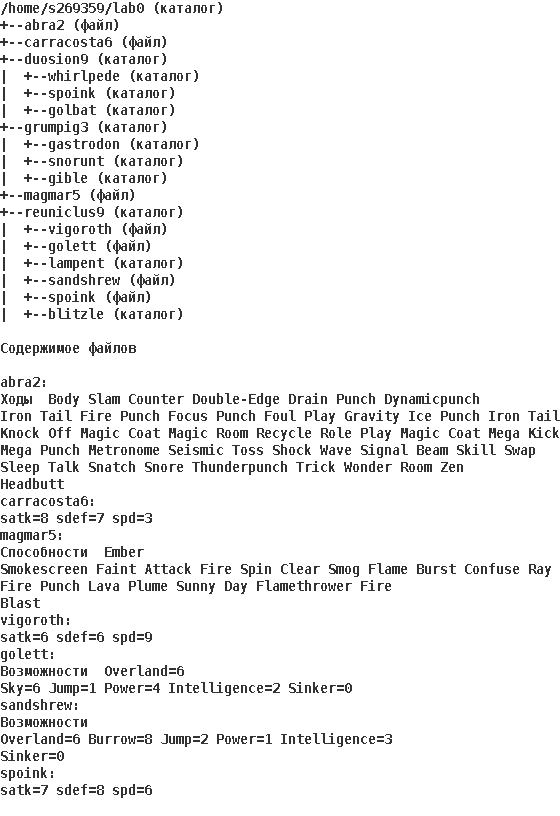
\includegraphics[width=400px, left]{tree.png}
	\pagebreak{}
	\item Set up file and directory permissions \texttt{chmod}, using different approaches.
	\begin{itemize}
		\item abra2: права 444
		\item carracosta6: права 666
		\item duosion9: владелец должен записывать директорию и переходить в нее; группа-владелец должна записывать директорию и переходить в нее; остальные пользователи должны читать директорию и переходить в нее
		\item whirlpede: права 550
		\item spoink: права 770
		\item golbat: владелец должен читать директорию и переходить в нее; группа-владелец должна только переходить в директорию; остальные пользователи должны записывать директорию и переходить в нее
		\item grumpig3: владелец должен записывать директорию и переходить в нее; группа-владелец должна читать, записывать директорию и переходить в нее; остальные пользователи должны читать директорию и переходить в нее
		\item gastrodon: владелец должен записывать директорию и переходить в нее; группа-владелец должна только переходить в директорию; остальные пользователи должны только переходить в директорию
		\item snorunt: права 317
		\item gible: rwx-wx-wx
		\item magmar5: права 066
		\item reuniclus9: владелец должен читать, записывать директорию и переходить в нее; группа-владелец должна записывать директорию и переходить в нее; остальные пользователи должны читать и записывать директорию
		\item vigoroth: права 444
		\item golett: владелец должен читать и записывать файл; группа-владелец должна записывать файл; остальные пользователи должны не иметь никаких прав
		\item lampent: владелец должен читать директорию и переходить в нее; группа-владелец должна только переходить в директорию; остальные пользователи должны записывать директорию и переходить в нее
		\item sandshrew: владелец должен не иметь никаких прав; группа-владелец должна читать файл; остальные пользователи должны читать файл
		\item spoink: права 440
		\item blitzle: r-x--x-wx
	\end{itemize}
	\item  Copy tree parts and create links with \texttt{cp} and \texttt{ln}, as well as with \texttt{cat} and io streams redirection.
	\begin{itemize}
		\item создать символическую ссылку c именем Copy\_91 на директорию reuniclus9 в каталоге lab0
		\item cоздать жесткую ссылку для файла abra2 с именем lab0/reuniclus9/golettabra
		\item скопировать файл carracosta6 в директорию lab0/grumpig3/snorunt
		\item скопировать содержимое файла abra2 в новый файл lab0/reuniclus9/vigorothabra
		\item cоздать символическую ссылку для файла magmar5 с именем\\ lab0/reuniclus9/vigorothmagmar
		\item объеденить содержимое файлов lab0/reuniclus9/golett, lab0/reuniclus9/golett, в новый файл lab0/abra2\_49
		\item скопировать рекурсивно директорию grumpig3 в директорию\\ lab0/grumpig3/snorunt
	\pagebreak{}
	\end{itemize}
	\item Using \texttt{cat}, \texttt{wc}, \texttt{ls}, \texttt{head}, \texttt{tail}, \texttt{echo}, \texttt{sort}, \texttt{grep} looks up and filters directory, files and data in it.
	\begin{itemize}
	\item Подсчитать количество строк содержимого файлов в директории grumpig3, отсортировать вывод по уменьшению количества, ошибки доступа перенаправить в файл в директории /tmp
	\item Вывести список имен и атрибутов файлов в директории duosion9, список отсортировать по убыванию размера, ошибки доступа перенаправить в файл в директории /tmp
	\item Рекурсивно вывести содержимое файлов с номерами строк из директории lab0, имя которых заканчивается на 'e', строки отсортировать по имени a->z, добавить вывод ошибок доступа в стандартный поток вывода
	\item Подсчитать количество строк содержимого файла carracosta6, результат записать в тот-же файл, ошибки доступа перенаправить в файл в директории /tmp
	\item Вывести рекурсивно список имен и атрибутов файлов в директории duosion9, список отсортировать по возрастанию количества жестких ссылок, ошибки доступа перенаправить в файл в директории /tmp
	\item Вывести рекурсивно список имен и атрибутов файлов в директории lab0, заканчивающихся на символ 't', список отсортировать по убыванию даты модификации файла, подавить вывод ошибок доступ
	\end{itemize}
	\item Remove files using rm and rmdir according following:
	\begin{itemize}
	\item Удалить файл abra2
	\item Удалить файл lab0/reuniclus9/golett
	\item удалить символические ссылки lab0/reuniclus9/vigorothmagm*
	\item удалить жесткие ссылки lab0/reuniclus9/golettab*
	\item Удалить директорию duosion9
	\item Удалить директорию lab0/grumpig3/gastrodon
	\end{itemize}
\end{enumerate}
\pagebreak{}
\section{Иерархия файлов после выполения п.3}
	Ниже приведен вывод команды \texttt{ls -lR} для директории  \texttt{lab0}. 
Для вывода полного дерева владельцу выдано право на чтение поддиректорий \texttt{duosion9}, \texttt{grumpig3},\\ \texttt{grumpig3/snorunt} и \texttt{grumpig3/gastrodon}. Вывод команды оставлен без изменений.\\
\small
\lstinputlisting[language={}, inputencoding=cp1251,numbers=left]{tree}
\large

\section{Возникающие ошибки}
\subsection*{п.3}
В ходе выполнения этого пункта возникает необходмость рекурсивно скопировать директорию \texttt{grumpig3} в свою поддиректорию \texttt{grumpig3/snorunt}, в ходе чего возникает ошибка:\\\\
	\texttt{cp: невозможно получить доступ к 'grumpig3/': Permission denied}\\\\
Для устранения данной ошибки и двух подобных трем поддирикториям необходмо выдать право на чтение:\\\\
\texttt{chmod u+r grumpig3\\
chmod u+r grumpig3/gastrodon\\
chmod u+r grumpig3/snorunt}\\
\\После выполнения этих операция появляется новая ошибка:
\\\\
\small
\texttt{cp: невозможно скопировать каталог 'grumpig3/' в самого себя, 'grumpig3/snorunt/grumpig3}
\large
\\\\
Действительно, если утилита cp бы начала рекурсивно копировать директорию в свою поддиректорию то этот цикл бы никогда не кончился. Приводим очевидное решение: остановимся на первом ветке рекурсии. Скопирем директорию \texttt{grumpig3} во временную \texttt{/tmp} и затем из временной переместим в  \texttt{grumpig3/snorunt/}:\\\\
\texttt{chmod u+r grumpig3\\
chmod u+r grumpig3/gastrodon\\
chmod u+r grumpig3/snorunt\\
cp -R grumpig3 /tmp/grumpig3\\
cp -R /tmp/grumpig3 grumpig3/snorunt \&\& rm -rf /tmp/grumpig3}\\\\
В полной версии скрипта после этих операций директориям также возвращаются исходные права.
\subsection*{п.4}
Почти на всех подпунктах этого задания возникают ошибки доступа, аналогичные первой ошибке из разбора п.3, в полной версии скрипта необходимые
 права выдаются и забираются после выполнения каджого подпункта.
\subsection*{п.5}
При попытке рекурсивного удаления директории duosion9 возникает ошибка:\\\\
\texttt{rm: невозможно удалить 'duosion9': Permission denied}\\\\
Для рекурсивного удаления директории требуются права на чтение:\\\\
\texttt{chmod u+r duosion9/}\\\\
\section{Вывод скрипта}
\texttt{-rw--w---- 1 s269359 studs 79 сент. 29 19:49 ./reuniclus9/golett}\\\\
\section{Скрипт}
Все решение разделено для структурирования на несколько скриптов.
\begin{enumerate}
\item \texttt{lab0.sh} - запуск всех скриптов в нужном порядке
\item \texttt{tree.sh} - создание дерева каталогов (п.1 задания)
\item \texttt{content.sh} - заполнение файлов содержанием (п.1 задания)
\item \texttt{perm.sh} - выдача прав (п.2 задания)
\item \texttt{cp\_ln.sh} - п.3 задания
\item  \texttt{fourth\_stage.sh} - п.4 задания
\item  \texttt{rm.sh} - п.5 задания
\small
\subsection{lab0.sh}
\lstinputlisting[language={bash},numbers=left]{scripts/lab0.sh}
\pagebreak{}
\subsection{tree.sh}
\lstinputlisting[language={bash},numbers=left]{scripts/tree.sh}
\subsection{content.sh}
\lstinputlisting[language={bash},inputencoding=cp1251,numbers=left]{scripts/content.sh}
\subsection{perm.sh}
\lstinputlisting[language={bash},numbers=left]{scripts/perm.sh}
\subsection{cp\_ln.sh}
\lstinputlisting[language={bash},numbers=left]{scripts/cp_ln.sh}
\pagebreak{}
\subsection{fourth stage.sh}
\lstinputlisting[language={bash},numbers=left]{scripts/fourth_stage.sh}
\pagebreak{}
\subsection{rm.sh}
\lstinputlisting[language={bash},numbers=left]{scripts/rm.sh}
\section{Содержание файла с ошибками в /tmp}
\texttt{find: cannot read dir grumpig3/snorunt: Permission denied\\
find: cannot read dir grumpig3/gastrodon: Permission denied}
\large
\section{Вывод}
В ходе это лаборатороной работы я научился работать с основными командами, утилитами и фильтрами системы Unix, познакомился с
различными ключами, написанием скриптов для командной оболочки.
\end{enumerate}
\end{document}